%%%%%%%%%%%%%%%%%%%%%%%%%%%%%%%%%%%%%%%%%
% University/School Laboratory Report
% LaTeX Template
% Version 3.1 (25/3/14)
%
% This template has been downloaded from:
% http://www.LaTeXTemplates.com
%
% Original author:
% Linux and Unix Users Group at Virginia Tech Wiki 
% (https://vtluug.org/wiki/Example_LaTeX_chem_lab_report)
%
% License:
% CC BY-NC-SA 3.0 (http://creativecommons.org/licenses/by-nc-sa/3.0/)
%
%%%%%%%%%%%%%%%%%%%%%%%%%%%%%%%%%%%%%%%%%

%----------------------------------------------------------------------------------------
%	PACKAGES AND DOCUMENT CONFIGURATIONS
%----------------------------------------------------------------------------------------

\documentclass{article}
\usepackage[version=3]{mhchem} % Package for chemical equation typesetting
%\usepackage{siunitx}  Provides the \SI{}{} and \si{} command for typesetting SI units
\usepackage{graphicx} % Required for the inclusion of images
\usepackage{natbib} % Required to change bibliography style to APA
\usepackage{amsmath, amssymb, amsthm, verbatim, amsfonts, amstext}
\usepackage{algorithms}
\usepackage{algorithmic}
\usepackage{ucs}
\usepackage[utf8]{inputenc}
\usepackage{multirow}
\usepackage[portuges,brazilian,english]{babel}
\DeclareMathOperator*{\argmin}{arg\,min}
\usepackage[scientific-notation=true]{siunitx}
\sisetup{round-precision=4,round-mode=figures,scientific-notation=true}
\usepackage{adjustbox}
\usepackage{caption}
\usepackage{subcaption}

\usepackage{float}

\setlength\parindent{0pt} % Removes all indentation from paragraphs

\renewcommand{\labelenumi}{\alph{enumi}.} % Make numbering in the enumerate environment by letter rather than number (e.g. section 6)

%\usepackage{times} % Uncomment to use the Times New Roman font

%----------------------------------------------------------------------------------------
%	DOCUMENT INFORMATION
%----------------------------------------------------------------------------------------

\title{Análise do $K$-NN e DMC para tarefa de classificação} % Title

\author{Leandro \textsc{Marinho}} % Author name

\date{27 de fevereiro de 2015} % Date for the report

\begin{document}

\maketitle % Insert the title, author and date

\begin{center}
\begin{tabular}{l r}
Mestrado em Ciência da Computação do \\
Instituto Federal do Ceará (PPGCC/IFCE) \\
Disciplina: Aprendizagem de Máquina \\
Professor: Dr. Ajalmar % Instructor/supervisor
\end{tabular}
\end{center}

% If you wish to include an abstract, uncomment the lines below
% \begin{abstract}
% Abstract text
% \end{abstract}

%----------------------------------------------------------------------------------------
%	SECTION 1
%----------------------------------------------------------------------------------------

\section{Introdução}

Aprendizado de máquina é um subcampo da inteligência artificial, dedicado ao desenvolvimento de algoritmos e técnicas que permitam o computador aprender, isto é, que permitam o computador aperfeiçoar seu desempenho em alguma tarefa.

De acordo com os conceitos/padrões a serem aprendidos e a disponibilidade de dados para treinamento, pode-se separar em dois tipos de aprendizado, os quais são conhecidos como paradigmas do aprendizado de máquina: aprendizado supervisionado e não supervisionado.

Este relatório tem como objetivo mostrar o comportamento do $K$-vizinhos mais próximos ($K$-NN, \textit{k-Nearest Neighbour}) e Distancia Mínima aos Centroides (DMC), algoritmos de aprendizagem supervisionada, para a tarefa de classificação.
 

%To determine the atomic weight of magnesium via its reaction with oxygen and to study the stoichiometry of the reaction (as defined in \ref{definitions}):
%
%\begin{center}\ce{2 Mg + O2 -> 2 MgO}\end{center}

\subsection{K-NN}
O algoritmo $K$-NN baseia-se no princípio de que as instâncias dentro de um conjunto de dados, em geral, estarão próximas de outras com propriedades semelhantes \cite{Cover:2006}. A classificação de um exemplo não rotulado, ou seja, cuja classe não é conhecida é determinado através da observação da classe dos seus vizinhos mais próximos. O $K$-NN localiza os $K$ exemplos mais próximos à instância de consulta e determina a sua classe, identificando o rótulo da classe mais freqüente. O classificador é apresentado no Algoritmo \ref{alg:knn}

\begin{algorithm}[!h]
\caption{Algoritmo Vizinho Mais Próximo (\textit{Nearest Neighbor}, NN)}\label{alg:knn}
\begin{algorithmic}[1]
\STATE Armazenar os exemplos em uma tabela.%
\STATE Seja $x_{novo}$ um vetor cuja classe é desconhecida, ou seja:
\begin{equation*}
Classe(x_{novo}) = ?
\end{equation*}
%
\STATE Encontrar na tabela os $K$ vetores mais próximo de $x_{novo}$.%
\STATE Seja $C_K$ a classe a que pertence a maioria dos K vetores.%
\STATE Atribuir a $x_{novo}$ a classe da maioria dos $K$ vetores, ou seja:
\begin{equation*}
Classe(x_{novo}) = C_K
\end{equation*}
%
\STATE Se a classificação for correta incluir $x_{novo}$ na tabela.
\end{algorithmic}
\end{algorithm}


\subsection{DMC}
O algoritmo DMC funciona de forma similar ao do Vizinho Mais Próximo. No entanto, cada classe passa a ter um único vetor que a representa, chamado de centróide. Dessa forma, não há necessidade de armazenar todos os exemplos de uma classe o que nos leva a uma economia de memória. O centróide de uma classe é o seu vetor médio; ou seja, a média dos exemplos daquela classe. Assim, pode-se dizer que o centróide de uma classe é um modelo que representa aquela classe. Um resumo do funcionamento do classificador é mostrado no Algoritmo \ref{alg:dmc}

\begin{algorithm}[!h]
\caption{Algoritmo Distância Mínima aos Centróides (DMC).}\label{alg:dmc}
\begin{algorithmic}[1]
\STATE Armazenar apenas os centróides das classes em uma tabela.%
\STATE Seja $x_{novo}$ um vetor cuja classe é desconhecida, ou seja:
\begin{equation*}
Classe(x_{novo}) = ?
\end{equation*}
%
\STATE Procurar na tabela o centróide mais próximo de $x_{novo}$.%
\STATE Chamar de $C_j$ o centróide mais próximo de $x_{novo}$.%
\STATE Atribuir a $x_{novo}$ a mesma classe de centróide mais próximo, ou seja:
\begin{equation*}
Classe(x_{novo}) = Classe(C_j)
\end{equation*}
%
\STATE Se a classificação for correta, usar $x_{novo}$ para recalcular $C_j$.
\end{algorithmic}
\end{algorithm}

%\begin{description}
%\item[Stoichiometry]
%The relationship between the relative quantities of substances taking part in a reaction or forming a compound, typically a ratio of whole integers.
%\item[Atomic mass]
%The mass of an atom of a chemical element expressed in atomic mass units. It is approximately equivalent to the number of protons and neutrons in the atom (the mass number) or to the average number allowing for the relative abundances of different isotopes.
%\end{description} 
 
%----------------------------------------------------------------------------------------
%	SECTION 2
%----------------------------------------------------------------------------------------

\section{Metodologia}

O $K$-NN e o DMC foram testados com a base de dados Iris do repositório UCI \cite{Lichman:2013}. Ela é composta por 4 atributos (largura e tamanho da sépala e pétala), 3 classes (Versicolor, Setosa e Virgínica)  e 150 instâncias (50 de cada uma das classes). Os dados foram particionados, aleatoriamente, em conjuntos de teste (20\%) e treinamento (80\%).

Primeiramente, foram escolhidos 25 valores (1 : 1 : 25)  de vizinhos para o $K$-NN. Dentre estes, o que obteve a maior acurácia média foi comparado ao DMC através da matriz de confusão e do gráficos de superfície de decisão. Por último, foram realizadas combinações entre os atributos com intuito de verificar sua influência na tarefa de classificação. Todos os experimentos foram repetidos 500 vezes para o cálculo da média e desvio padrão. 


%\begin{tabular}{ll}
%Mass of empty crucible & \SI{7.28}{\gram}\\
%Mass of crucible and magnesium before heating & \SI{8.59}{\gram}\\
%Mass of crucible and magnesium oxide after heating & \SI{9.46}{\gram}\\
%Balance used & \#4\\
%Magnesium from sample bottle & \#1
%\end{tabular}


%----------------------------------------------------------------------------------------
%	SECTION 3
%----------------------------------------------------------------------------------------

%\section{Sample Calculation}
%
%\begin{tabular}{ll}
%Mass of magnesium metal & = \SI{8.59}{\gram} - \SI{7.28}{\gram}\\
%& = \SI{1.31}{\gram}\\
%Mass of magnesium oxide & = \SI{9.46}{\gram} - \SI{7.28}{\gram}\\
%& = \SI{2.18}{\gram}\\
%Mass of oxygen & = \SI{2.18}{\gram} - \SI{1.31}{\gram}\\
%& = \SI{0.87}{\gram}
%\end{tabular}
%
%Because of this reaction, the required ratio is the atomic weight of magnesium: \SI{16.00}{\gram} of oxygen as experimental mass of Mg: experimental mass of oxygen or $\frac{x}{1.31}=\frac{16}{0.87}$ from which, $M_{\ce{Mg}} = 16.00 \times \frac{1.31}{0.87} = 24.1 = \SI{24}{\gram\per\mole}$ (to two significant figures).

%----------------------------------------------------------------------------------------
%	SECTION 4
%----------------------------------------------------------------------------------------

\section{Resultados e Discussões}

\subsection{Base de dados}
A Figura \ref{img:iris} mostra a disposição das classes combinando 2 atributos por vez. As classes Versicolor e Virgínica estão sobrepostas em todos os gráficos. A relação entre os atributos tamanho e largura da pétala foi uma das que proporcionaram uma separação maior entre a classe Setosa das demais no espaço bidimensional.

\begin{figure}[!h]
\begin{center}
\makebox[\textwidth][c]{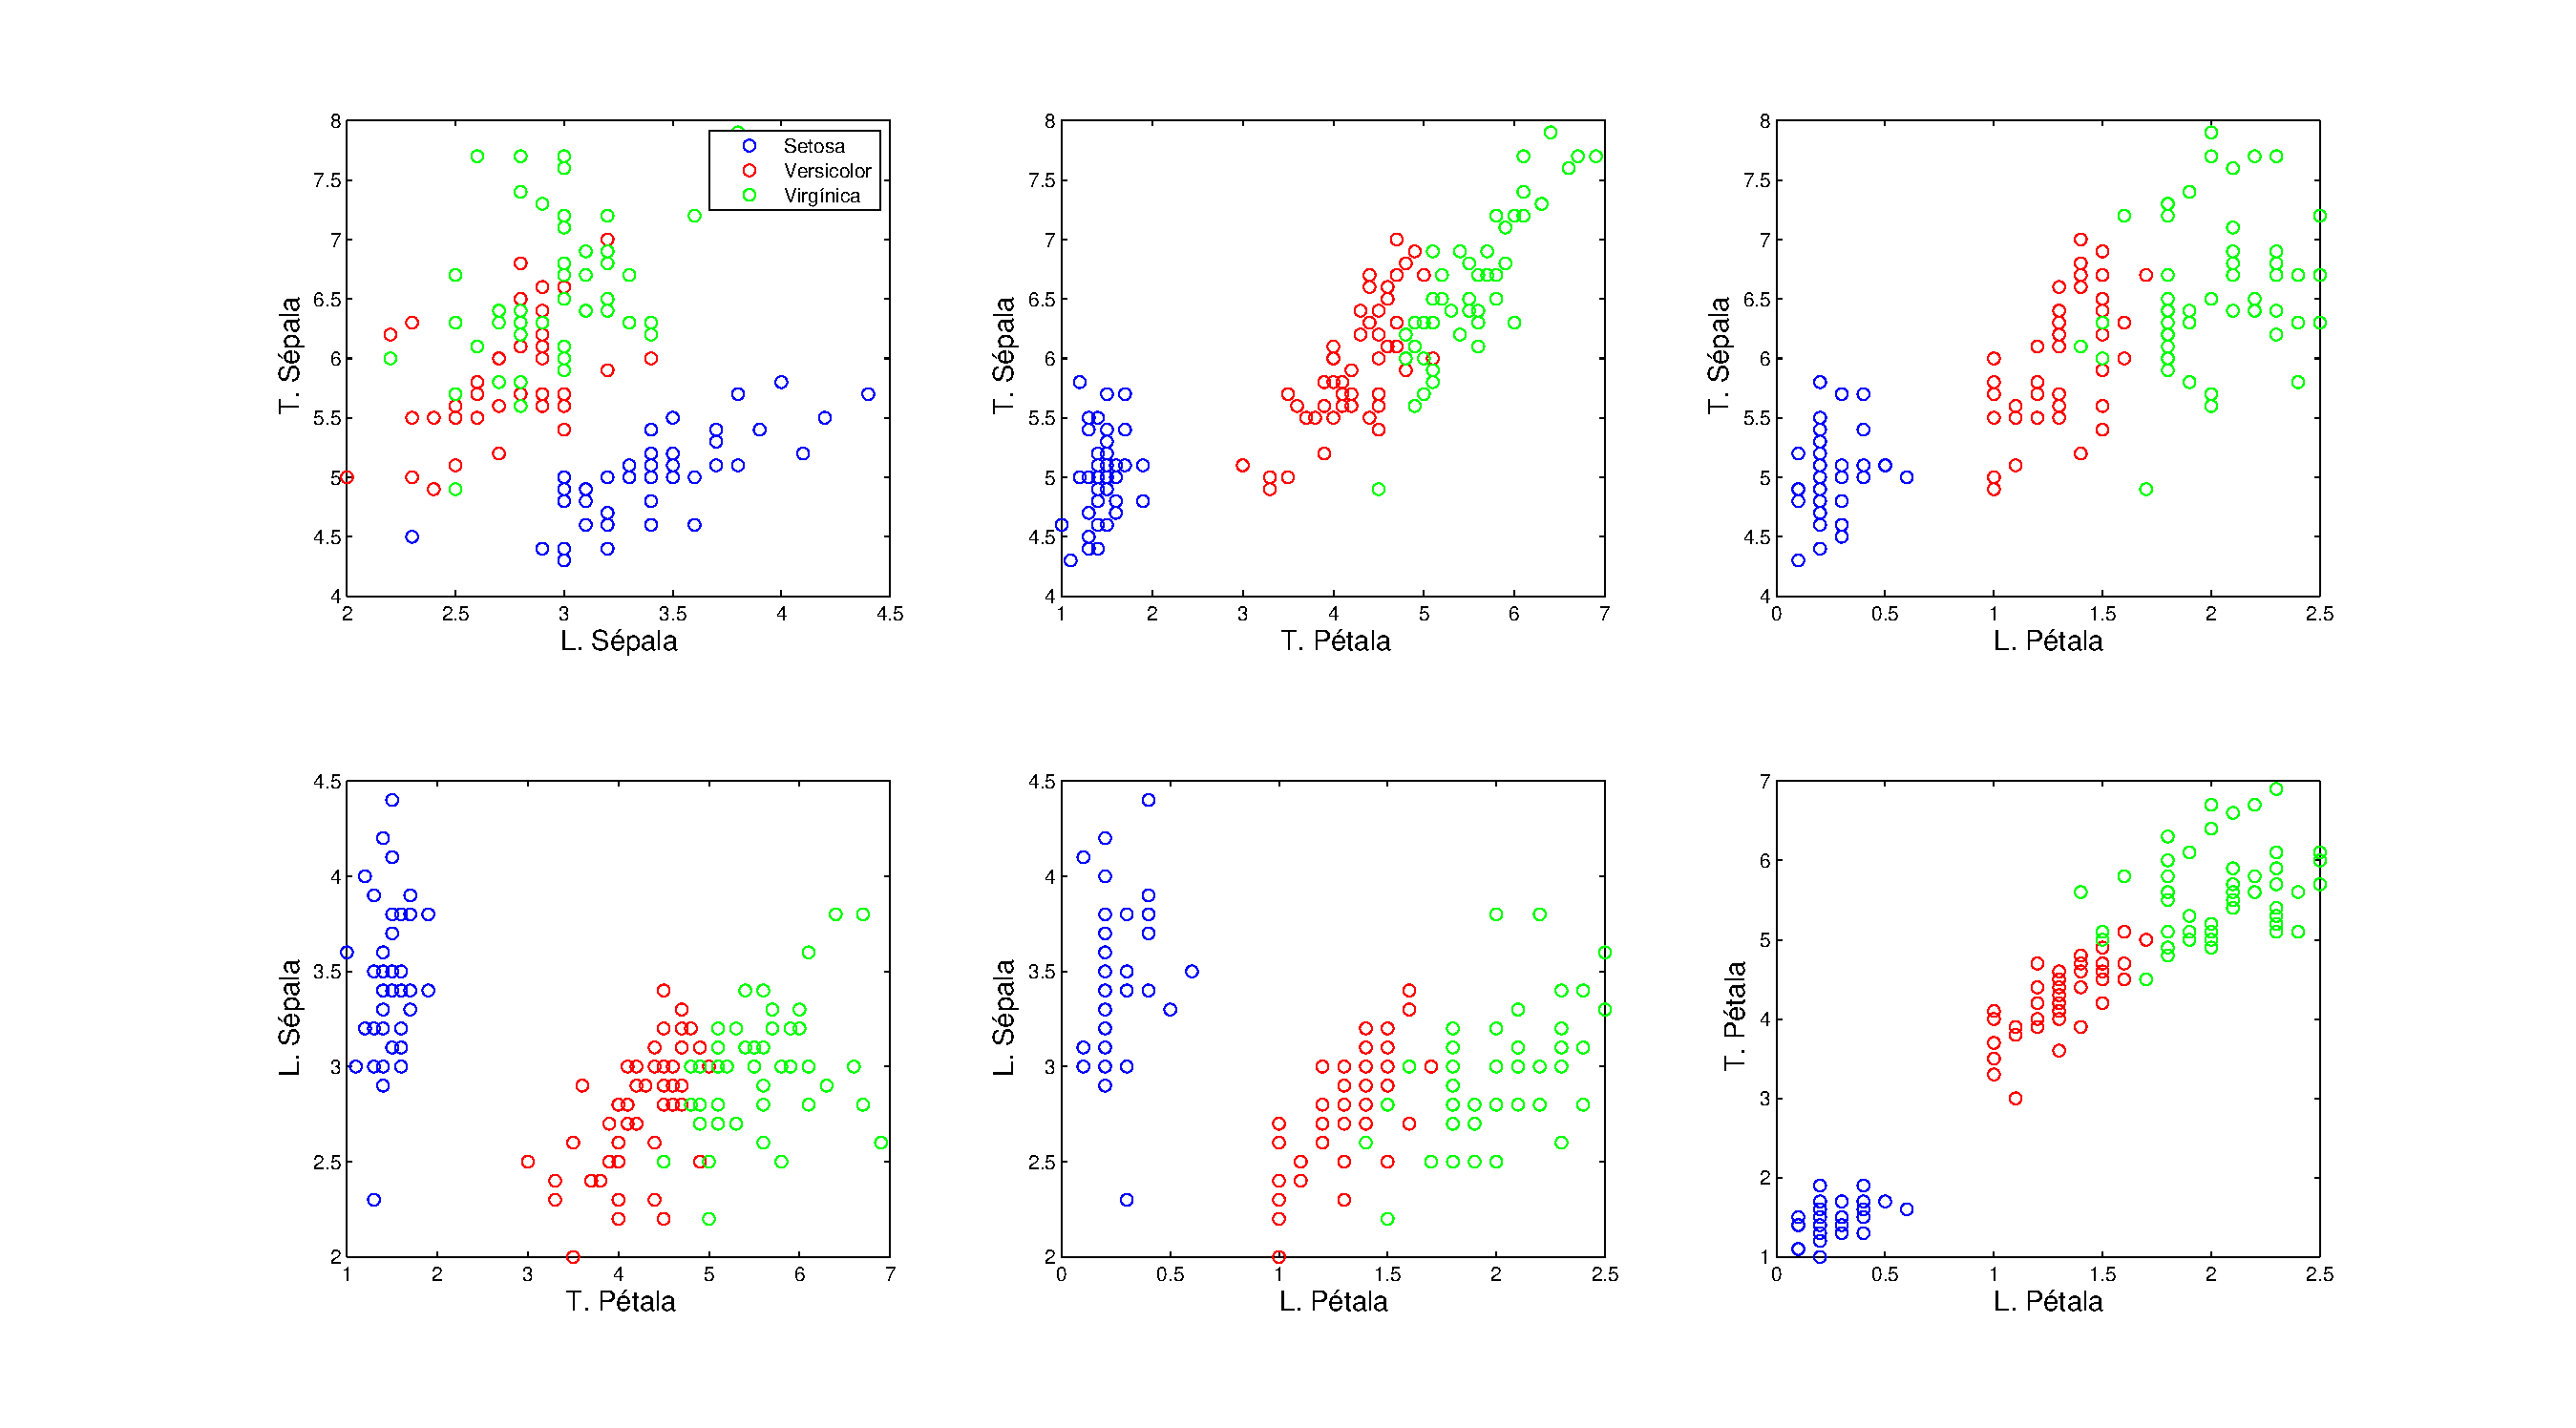
\includegraphics[width=1.6\textwidth]{iris.eps}}
\caption{Conjunto de dados Iris}
\label{img:iris}
\end{center}
\end{figure}

\subsection{KNN e DMC}
A Tabela \ref{tab:knn} mostra a média e o desvio padrão da taxa de acerto dos $K$-NNs utilizando todos atributos da base de dados. Como pode ser observado, o $13$-NN tem a maior acurácia. Ou seja, um número pequeno de vizinhos pode diminuir a taxa de acerto do classificador, assim como, um grande número de vizinhos.

%A média e o desvio padrão do $K$-NN são representados nas colunas 2 e 3 e as do $K$-NN* nas colunas 4 e 5. A primeira coluna indicia o número de vizinhos.

\begin{table}[!h]
	\centering
	\vspace{0.5cm}
\begin{tabular}{lllll}
\hline
K  & Média (\%) & Desvio Padrão \\ \hline \hline

1  & 95,6867 & \num{0,0399072999912622} \\ \hline
2  & 94,6600 & \num{0,0322030594359765} \\ \hline
3  & 96,0867 & \num{0,0161015297179883} \\ \hline
4  & 95,7400 & \num{0,0378430808131698} \\ \hline
5  & 96,4667 & \num{0,0331476308670584} \\ \hline
6  & 96,1400 & \num{0,0306312194490894} \\ \hline
7  & 96,4933 & \num{0,0351364184463153} \\ \hline
8  & 96,4200 & \num{0,0449965705140369} \\ \hline
9  & 96,5400 & \num{0,0175682092231577} \\ \hline
10 & 96,3000 & \num{0,0417221852344857} \\ \hline
11 & 96,8400 & \num{0,0391262596925756} \\ \hline
12 & 96,5467 & \num{0,0291865011923638} \\ \hline
13 & \textbf{97,0000} & \num{0,0224982852570184} \\ \hline
14 & 96,4467 & \num{0,0316227766016838} \\ \hline
15 & 96,7200 & \num{0,0291865011923638} \\ \hline
16 & 96,3800 & \num{0,0224982852570184} \\ \hline
17 & 96,8600 & \num{0,0245954929124207} \\ \hline
18 & 96,1800 & \num{0,0316227766016838} \\ \hline
19 & 96,2200 & \num{0,0316227766016838} \\ \hline
20 & 95,5800 & \num{0,0316227766016838} \\ \hline
21 & 95,6200 & \num{0,0316227766016838} \\ \hline
22 & 95,2600 & \num{0,0316227766016838} \\ \hline
23 & 94,9267 & \num{0,0316227766016838} \\ \hline
24 & 94,6467 & \num{0,0316227766016838} \\ \hline
25 & 94,8933 & \num{0,0316227766016838} \\ \hline

\end{tabular}
\caption{Média e desvio padrão da taxa de acerto do $K$-NN.}\label{tab:knn}
\end{table}

Analisando o resultado anterior através da Figura \ref{img:knn}, é possível ver que o $K$-NN tem uma discreta melhora da acurácia com o aumento do número de vizinhos, em seguida, este valor começa a diminuir.

\begin{figure}[H]
\begin{center}
	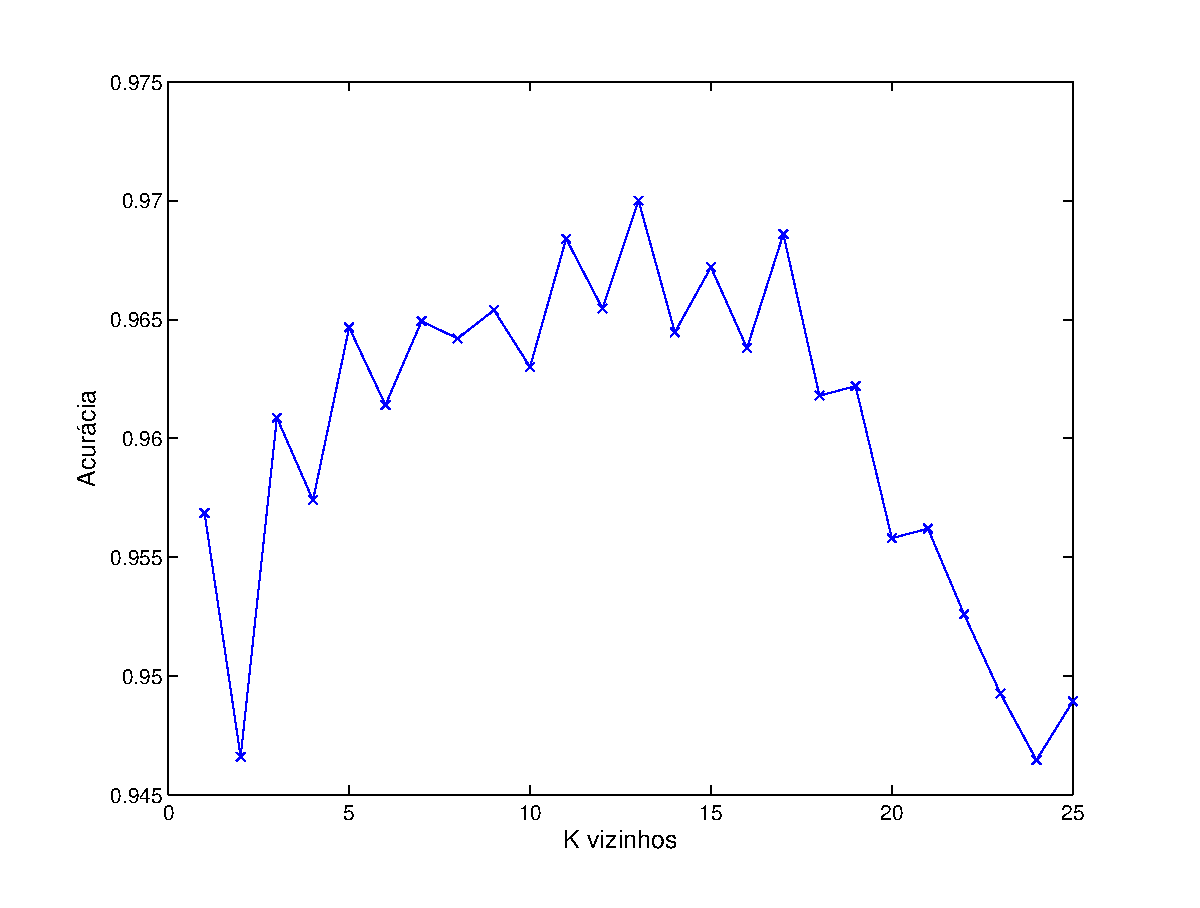
\includegraphics[scale=0.6]{knn.eps}
	\caption{Taxa de acerto dos K-NNs pelo número de vizinhos.}
	\label{img:knn}
	\end{center}
\end{figure}

A Tabela \ref{tab:knn_dmc} relaciona o método DMC com o $13$-NN, o $K$-NN com maior taxa de acerto da Tabela \ref{img:knn}. A comparação entre o $13$-NN e o DMC foi realizada separadamente com objetivo de selecionar o mesmo conjunto de treinamento e teste. A acurácia do DMC foi um pouco menor que a do $13$-NN. No entanto, é importante ressaltar que o custo computacional do DMC é menor.

\begin{table}[h]
	\centering
	\vspace{0.5cm}
\begin{tabular}{lllll}
\hline
  & Média (\%) & Desvio Padrão \\ \hline
13-NN & 96,333 & \num{0,029497309940035} \\ \hline
DMC & 92,186 & \num{0,047536319014761} \\ \hline
\end{tabular}
\caption{Média e desvio padrão da taxa de acerto do $K$-NN e DMC.}\label{tab:knn_dmc}
\end{table}

%Uma ferramenta importante para a avaliação da qualidade dos resultados obtidos é a matriz de confusão. Ela é uma matriz quadrada cuja dimensão é igual ao número de classes. Cada coluna da matriz indica a classe desejada e cada linha a classe estimada pelo classificador. Um dado elemento $C_{i,j}$ de uma matriz de confusão indica o número de elementos da classe $j$ que foram classificados como sendo da classe $i$. 

Uma ferramenta importante para a avaliação da qualidade dos resultados obtidos é a matriz de confusão. Ela é uma matriz quadrada cuja dimensão é igual ao número de classes. Sua diagonal principal exibe o número de acertos para as classes analisadas. Foram escolhidas as matrizes com a taxa de acerto mais próxima da acurácia média. 

Na matriz de confusão da Tabela \ref{tab:matriz_knn_dmc}, das 10 amostras Versicolor reais, o $13$-NN predisse que 1 era Virgínica, acertando as duas outras classes. O DMC errou ao tentar classificar duas amostras da classe Versicolor  e uma da Virgínica. Como esperado, a classe Setosa teve a maior taxa de acerto nos dois métodos.

\begin{table}[h]
\begin{tabular}{|l|l|l|l|l|l|l|}
\hline
Métodos    & \multicolumn{3}{c|}{\textbf{K-NN}} & \multicolumn{3}{c|}{\textbf{DMC}} \\ \hline
Classes    & Setosa  & Versicolor  & Virgínica  & Setosa  & Versicolor  & Virgínica \\ \hline
Setosa     & 7       & 0           & 0          & 7       & 0           & 0         \\ \hline
Versicolor & 0       & 9           & 1          & 0       & 8           & 2         \\ \hline
Virgínica  & 0       & 0           & 13         & 0       & 1           & 11        \\ \hline
\end{tabular}
\caption{Matrizes de confusão do K-NN e DMC}\label{tab:matriz_knn_dmc}
\end{table}

\subsection{Superfície de Decisão}
Foram realizadas combinações de atributos para encontrar superfícies de decisão para cada classificador no espaço bidimensional. É possível observar através da Figura \ref{img:knn_sd} que o 13-NN consegue uma boa separação entre as três classes na maioria dos gráficos, apresentando regiões desconexas da classe Versicolor no primeiro (largura e tamanho da sépala).

%É possível observar através da Figura \ref{img:knn_sd} que os atributos tamanho e largura da pétala (último gráfico) conseguem uma melhor separação da classe Setosa das demais utilizando o 13-NN. A largura e tamanho da sépala (primeiro gráfico) proporcionam uma maior sobreposição das classes.

\begin{figure}[!h]
\begin{center}
\makebox[\textwidth][c]{\includegraphics[width=1.6\textwidth]{knn_sd.eps}}
\caption{Superfícies de decisão do 13-NN com a Iris.}
\label{img:knn_sd}
\end{center}
\end{figure}

A Figura \ref{img:dmc_sd} mostra as superfícies de decisão do DMC. Assim como na Figura \ref{img:knn_sd}, os atributos tamanho e largura da pétala destacaram melhor a classe Setosa beneficiando a tarefa de classificação. Em contrapartida, a largura e tamanho da sépala tornaram as classes mais sobrepostas. 

\begin{figure}[!h]
\begin{center}
\makebox[\textwidth][c]{\includegraphics[width=1.6\textwidth]{dmc_sd.eps}}
\caption{Superfícies de decisão do DMC com a Iris.}
\label{img:dmc_sd}
\end{center}
\end{figure}

Uma observação importante é da flexibilidade nas separações entre as regiões utilizando o DMC e o 13-NN. Analisando, por exemplo, o segundo gráfico das Figuras \ref{tab:knn_dmc} e \ref{img:dmc_sd} é possível ver que o 13-NN consegue incluir mais amostras da classe Versicolor comparado ao DMC. Essa propriedade permitiu uma melhora na acurácia como visto nos experimentos anteriores.

\subsection{Combinações dos Atributos}
Gerou-se combinações dos atributos com objetivo de mostrar sua influência na tarefa de classificação. Os experimentos foram executados 500 vezes para o cálculo da média e desvio padrão utilizando o DMC e o 13-NN. Os valores 1,2,3 e 4 apresentados nas tabelas a seguir correspondem aos atributos tamanho da sépala, largura da sépala, tamanho da pétala, largura da pétala. Assim, no campo atributo de cada tabela são apresentados os atributos utilizados na combinação. Os resultados são apresentados nas tabelas \ref{tab:combinacao_4} - \ref{tab:combinacao_total}.

\begin{table}[!h]
	\centering
	\vspace{0.5cm}
\begin{tabular}{l|l|l|l|l|}
\cline{2-5}
                                & \multicolumn{2}{c|}{13-NN} & \multicolumn{2}{c|}{DMC}   \\ \hline
\multicolumn{1}{|l|}{Atributos} & Média (\%) & Desvio Padrão & Média (\%) & Desvio Padrão \\ \hline
\multicolumn{1}{|l|}{1, 2, 3, 4} & 96,333 & \num{0,029497309940035} & 92,186 & \num{0,047536319014761} \\ \hline
\end{tabular}
\caption{Combinação dos atributos tomados quatro-a-quatro. Ou seja, utilizando todos os atributos.}\label{tab:combinacao_4}
\end{table}

Pode-se verificar na Tabela \ref{tab:combinacao_3} que a acurácia do $K$-NN aumenta com a ausência do atributo 1. No entanto, os valores das médias são estatisticamente semelhantes, principalmente, quando se utilizam todos os atributos. O aumento da acurácia do DMC é mais significativa sem esse atributo.

\begin{table}[!h]
	\centering
	\vspace{0.5cm}
\begin{tabular}{l|l|l|l|l|}
\cline{2-5}
                                & \multicolumn{2}{c|}{13-NN} & \multicolumn{2}{c|}{DMC}   \\ \hline
\multicolumn{1}{|l|}{Atributos} & Média (\%) & Desvio Padrão & Média (\%) & Desvio Padrão \\ \hline
\multicolumn{1}{|l|}{1, 2, 3} & 94,440 & \num{0,037360} & 88,693 & \num{0,052103}       \\ \hline
\multicolumn{1}{|l|}{1, 2, 4} & 94,960 & \num{0,037212} & 86,453 & \num{0,056938}       \\ \hline
\multicolumn{1}{|l|}{2, 3, 4} & 96,693 & \num{0,029843} & 95,400 & \num{0,034861}       \\ \hline
\end{tabular}
\caption{Combinação dos atributos tomados três-a-três.}\label{tab:combinacao_3}
\end{table}

Pode-se verificar na Tabela \ref{tab:combinacao_2} que a combinação dos atributos 1 e 2 diminuem a acurácia de ambos classificadores. A diferença entre os demais ficaram próximas.

\begin{table}[!h]
	\centering
	\vspace{0.5cm}
\begin{tabular}{l|l|l|l|l|}
\cline{2-5}
                                & \multicolumn{2}{c|}{13-NN} & \multicolumn{2}{c|}{DMC}   \\ \hline
\multicolumn{1}{|l|}{Atributos} & Média (\%) & Desvio Padrão & Média (\%) & Desvio Padrão \\ \hline
\multicolumn{1}{|l|}{1, 2} & 77,953 & \num{0,068682} & 80,807 & \num{0,061484}       \\ \hline
\multicolumn{1}{|l|}{1, 3} & 94,460 & \num{0,037212} & 89,453 & \num{0,056938}       \\ \hline
\multicolumn{1}{|l|}{1, 4} & 94,993 & \num{0,029843} & 92.586 & \num{0.058469}       \\ \hline
\multicolumn{1}{|l|}{2, 3} & 94,766 & \num{0,029843} & 93,400 & \num{0,034861}       \\ \hline
\multicolumn{1}{|l|}{2, 4} & 95,386 & \num{0,035131} & 95,400 & \num{0,028161}       \\ \hline
\multicolumn{1}{|l|}{3, 4} & 96,053 & \num{0,029843} & 96,293 & \num{0,031362}       \\ \hline

\end{tabular}
\caption{Combinação dos atributos tomados dois-a-dois.}\label{tab:combinacao_2}
\end{table}

Na Tabela \ref{tab:combinacao_total} é apresentado um resumo dos piores resultados obtidos desde o uso de todos atributos até as combinações de atributos tomados dois-a-dois. Com base nos resultados apresentados, pode-se inferir que a escolha separada dos atributos 1 e 2 (tamanho da sépala, largura da sépala) proporcionam uma queda na acurácia dos classificadores.

\begin{table}[!h]
	\centering
	\vspace{0.5cm}
\begin{tabular}{l|l|l|l|l|}
\cline{2-5}
                                & \multicolumn{2}{c|}{13-NN} & \multicolumn{2}{c|}{DMC}   \\ \hline
\multicolumn{1}{|l|}{Atributos} & Média (\%) & Desvio Padrão & Média (\%) & Desvio Padrão \\ \hline
\multicolumn{1}{|l|}{1, 2} & 77,953 & \num{0,068682} & 80,807 & \num{0,061484}       \\ \hline
\multicolumn{1}{|l|}{1, 2, 3} & 94,440 & \num{0,037360} & 88,693 & \num{0,052103}       \\ \hline
\multicolumn{1}{|l|}{1, 2, 3, 4} & 96,333 & \num{0,029497309940035} & 92,186 & \num{0,047536319014761} \\ \hline

\end{tabular}
\caption{Combinação dos atributos tomados dois-a-dois.}\label{tab:combinacao_total}
\end{table}


%\subsection{Redução de dimensionalidade}
%O termo dimensionalidade é atribuído ao número de características de uma representação de padrões, ou seja, a dimensão do espaço de características. As duas principais razões para que a dimensionalidade seja a menor possível são: custo de medição e precisão do classificador. Quando o espaço de características contém somente as características mais salientes, o classificador será mais rápido e ocupará menos memória. Além disso, quando o conjunto de exemplos de treinamento não é muito grande, um espaço de características pequeno pode evitar a maldição da dimensionalidade e propiciar pequenas taxas de erro ao classificador.  Importante lembrar que estes objetivos devem ser alcançados sem que se deteriore a capacidade de um classificador.
%
%Há dois propósitos relacionados com a redução da dimensionalidade: extração de características e seleção de características. Uma técnica bastante empregada na extração de características é o método PCA (\textit{Principal Component Analysis}). A Tabela expõe ...



%----------------------------------------------------------------------------------------
%	SECTION 5
%----------------------------------------------------------------------------------------

\section{Conclusões}

De acordo com os resultados, podemos concluir que o $K$-NN e o DMC apresentaram boa performance para o problema de classificação multiclasse. É importante ressaltar, também, que se o $K$ for muito pequeno, a classificação fica sensível a pontos de ruído. Em contrapartida, se o $K$ é muito grande, a vizinhança pode incluir elementos de outras classes, prejudicando, assim, o classificador. Outro ponto relevante, é que a taxa de acerto obtida com os dos algoritmos foram semelhantes.

O $K$-NN e o DMC tem como vantagem sua facilidade de implementação diante de ótimos resultados apresentados em alguns casos. Classificar um exemplo desconhecido com o $K$-NN pode ser um processo computacionalmente complexo, pois ele requer um cálculo de distância para cada exemplo de treinamento. Em contrapartida, o DMC trata desta questão armazenando apenas os centróides.

Foi observado através da análise de base de dados, do gráfico de superfície decisão e das combinações de atributos que a escolha dos atributos tamanho e largura da sépala, separadamente, diminuem a acurácia dos classificadores.

%The accepted value (periodic table) is \SI{24.3}{\gram\per\mole} \cite{Smith:2012qr}. The percentage discrepancy between the accepted value and the result obtained here is 1.3\%. Because only a single measurement was made, it is not possible to calculate an estimated standard deviation.
%
%The most obvious source of experimental uncertainty is the limited precision of the balance. Other potential sources of experimental uncertainty are: the reaction might not be complete; if not enough time was allowed for total oxidation, less than complete oxidation of the magnesium might have, in part, reacted with nitrogen in the air (incorrect reaction); the magnesium oxide might have absorbed water from the air, and thus weigh ``too much." Because the result obtained is close to the accepted value it is possible that some of these experimental uncertainties have fortuitously cancelled one another.

%----------------------------------------------------------------------------------------
%	SECTION 6
%----------------------------------------------------------------------------------------

%\section{Answers to Definitions}
%
%\begin{enumerate}
%\begin{item}
%The \emph{atomic weight of an element} is the relative weight of one of its atoms compared to C-12 with a weight of 12.0000000$\ldots$, hydrogen with a weight of 1.008, to oxygen with a weight of 16.00. Atomic weight is also the average weight of all the atoms of that element as they occur in nature.
%\end{item}
%\begin{item}
%The \emph{units of atomic weight} are two-fold, with an identical numerical value. They are g/mole of atoms (or just g/mol) or amu/atom.
%\end{item}
%\begin{item}
%\emph{Percentage discrepancy} between an accepted (literature) value and an experimental value is
%\begin{equation*}
%\frac{\mathrm{experimental\;result} - \mathrm{accepted\;result}}{\mathrm{accepted\;result}}
%\end{equation*}
%\end{item}
%\end{enumerate}

%----------------------------------------------------------------------------------------
%	BIBLIOGRAPHY
%----------------------------------------------------------------------------------------

\bibliographystyle{apalike}

\bibliography{sample}

%----------------------------------------------------------------------------------------


\end{document}